\documentclass[landscape]{article}
\usepackage[paperwidth=16in,paperheight=9in,margin=0.35in]{geometry}
\usepackage{amsmath}
\usepackage{sfmath}
\usepackage{tikz}
\usetikzlibrary{arrows.meta}

\pagestyle{empty}

\begin{document}
\begin{center}
  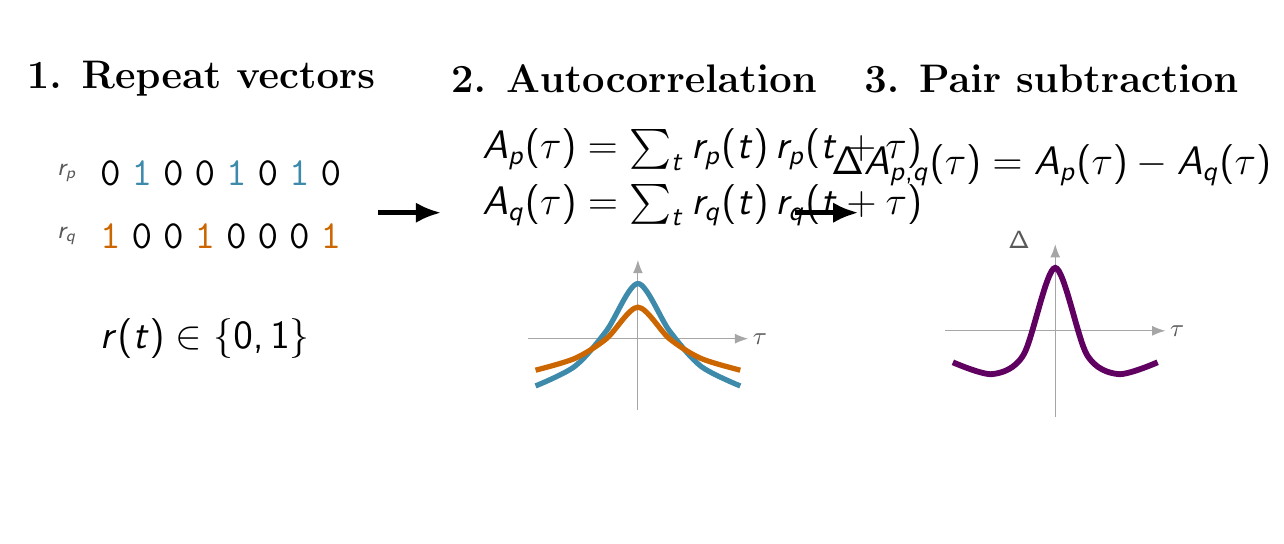
\begin{tikzpicture}[
      font=\sffamily,
      >=Latex,
      arrow/.style={line width=1.6pt,-{Latex[length=3.2mm,width=2.6mm]}},
      steptitle/.style={font=\bfseries\Large},
      eq/.style={font=\Large},
      note/.style={font=\small, text=black!65},
      bit/.style={font=\Large\ttfamily},
      onep/.style={font=\Large\ttfamily, text=cyan!65!black},
      oneq/.style={font=\Large\ttfamily, text=orange!80!black}
    ]

    \path[use as bounding box] (0,0) rectangle (15.6,6.2);

    % Step titles
    \node[steptitle] at (2.2,5.55) {1. Repeat vectors};
    \node[steptitle] at (7.7,5.55) {2. Autocorrelation};
    \node[steptitle] at (13.0,5.55) {3. Pair subtraction};

    % Step 1: explicit binary vectors
    \node[note, anchor=east] at (0.75,4.35) {$r_p$};
    \node[bit]  at (1.05,4.35) {0};
    \node[onep] at (1.45,4.35) {1};
    \node[bit]  at (1.85,4.35) {0};
    \node[bit]  at (2.25,4.35) {0};
    \node[onep] at (2.65,4.35) {1};
    \node[bit]  at (3.05,4.35) {0};
    \node[onep] at (3.45,4.35) {1};
    \node[bit]  at (3.85,4.35) {0};

    \node[note, anchor=east] at (0.75,3.55) {$r_q$};
    \node[oneq] at (1.05,3.55) {1};
    \node[bit]  at (1.45,3.55) {0};
    \node[bit]  at (1.85,3.55) {0};
    \node[oneq] at (2.25,3.55) {1};
    \node[bit]  at (2.65,3.55) {0};
    \node[bit]  at (3.05,3.55) {0};
    \node[bit]  at (3.45,3.55) {0};
    \node[oneq] at (3.85,3.55) {1};

    \node[eq] at (2.25,2.25) {$r(t)\in\{0,1\}$};

    % Arrow 1
    \draw[arrow] (4.45,3.85) -- (5.25,3.85);

    % Step 2: equations
    \node[eq, anchor=west] at (5.65,4.65)
    {$A_p(\tau)=\sum_t r_p(t)\,r_p(t+\tau)$};

    \node[eq, anchor=west] at (5.65,3.95)
    {$A_q(\tau)=\sum_t r_q(t)\,r_q(t+\tau)$};

    % Step 2: axes and curves
    \draw[black!35,->] (6.35,2.25) -- (9.15,2.25);
    \draw[black!35,->] (7.75,1.35) -- (7.75,3.25);
    \node[note] at (9.3,2.25) {$\tau$};

    \draw[cyan!65!black, line width=1.9pt]
    plot[smooth] coordinates {
      (6.45,1.65) (6.95,1.9) (7.35,2.35)
      (7.75,2.95) (8.15,2.35) (8.55,1.9) (9.05,1.65)
    };

    \draw[orange!80!black, line width=1.9pt]
    plot[smooth] coordinates {
      (6.45,1.85) (6.95,2.0) (7.35,2.25)
      (7.75,2.65) (8.15,2.25) (8.55,2.0) (9.05,1.85)
    };

    % Arrow 2
    \draw[arrow] (9.75,3.85) -- (10.55,3.85);

    % Step 3: subtraction equation
    \node[eq] at (13.0,4.45)
    {$\Delta A_{p,q}(\tau)=A_p(\tau)-A_q(\tau)$};

    % Step 3: axes and curve
    \draw[black!35,->] (11.65,2.35) -- (14.45,2.35);
    \draw[black!35,->] (13.05,1.25) -- (13.05,3.45);
    \node[note] at (14.6,2.35) {$\tau$};
    \node[note, anchor=east] at (12.85,3.5) {$\Delta$};

    \draw[violet!75!black, line width=2.1pt]
    plot[smooth] coordinates {
      (11.75,1.95) (12.25,1.8) (12.65,2.05)
      (13.05,3.15) (13.45,2.05) (13.85,1.8) (14.35,1.95)
    };

  \end{tikzpicture}
\end{center}
\end{document}